% You should title the file with a .tex extension (hw1.tex, for example)
\documentclass[a4paper, 11pt]{article}

\usepackage{amsmath}
\usepackage{amssymb}
\usepackage{fancyhdr}
\usepackage{graphicx}

\usepackage[margin=1in]{geometry}
\usepackage{tikz}
\usetikzlibrary{automata,positioning,arrows}
\newcommand{\question}[2] {\vspace{.25in} \hrule\vspace{0.5em}
	\noindent{\bf #1: #2} \vspace{0.5em}
	\hrule \vspace{.10in}}
\renewcommand{\part}[1] {\vspace{.10in} {\bf (#1)}}

\newcommand{\myname}{Possawat Sanorkam}
\newcommand{\myemail}{possawat2017@hotmail.com}
\newcommand{\myhwnum}{2}

\setlength{\parindent}{0pt}
\setlength{\parskip}{5pt plus 1pt}

\pagestyle{fancyplain}
\lhead{\fancyplain{}{\textbf{HW\myhwnum}}}      % Note the different brackets!
\rhead{\fancyplain{}{\myname\\ \myemail}}
\chead{\fancyplain{}{ICCS310}}

\begin{document}
	
	\medskip                        % Skip a "medium" amount of space
	% (latex determines what medium is)
	% Also try: \bigskip, \littleskip
	
	\thispagestyle{plain}
	\begin{center}                  % Center the following lines
		{\Large ICCS310: Assignment \myhwnum} \\
		\myname \\
		\myemail \\
		\today \\
	\end{center}
	
	\question{1}{Regex to NFA/DFA} %don't delete yet:(}
	
	\part{1} $a(abb)^* + b $
	
	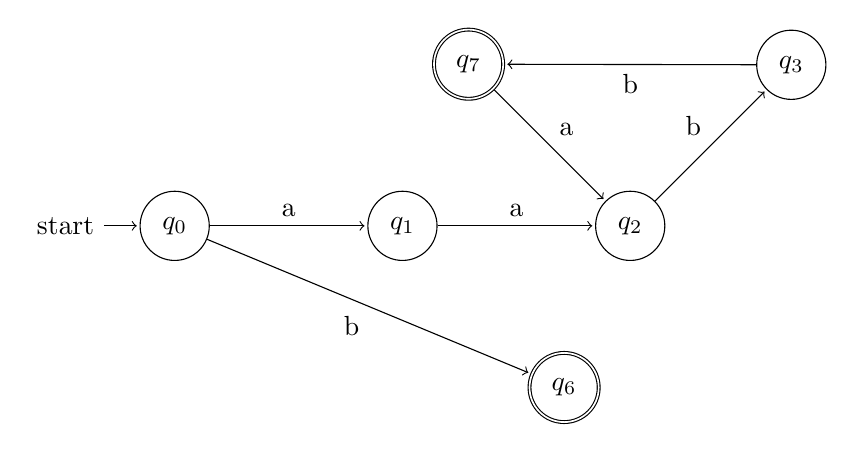
\begin{tikzpicture}[shorten >=1pt,node distance=2cm,auto] 
	\node[state,initial] (q_0)   {$q_0$}; 
	\node[state] (q_1) [ right=of q_0] {$q_1$}; 
	\node[state] (q_2) [ right=of q_1] {$q_2$}; 
	\node[state] (q_3) [above right=of q_2] {$q_3$}; 
	\node[state,accepting](q_6) [below right=of q_1] {$q_6$};	
	\node[state,accepting](q_7) [above left=of q_2] {$q_7$};
	\path[->] 
	(q_0) edge  node {a} (q_1)
	edge [swap] node {b} (q_6)
	(q_1) edge  node {a} (q_2)
	(q_2) edge  node {b} (q_3)
	(q_3) edge  node {b} (q_7)
	(q_7) edge  node {a} (q_2);

	\end{tikzpicture}
	
	\part{2} $(a + b)^* aa(a + b)^*$
	
	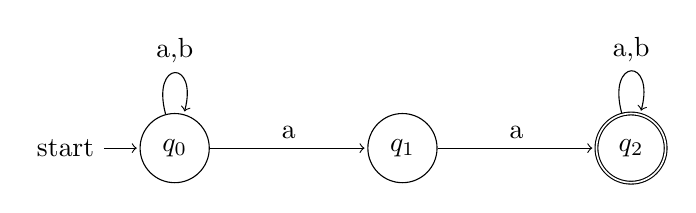
\begin{tikzpicture}[shorten >=1pt,node distance=2cm,auto] 
	\node[state,initial] (q_0)   {$q_0$}; 
	\node[state] (q_1) [right=of q_0] {$q_1$}; 
	\node[state,accepting](q_2) [right=of q_1] {$q_2$};
	\path[->] 
	(q_0) edge [loop above] node {a,b} ()
	edge  node {a} (q_1)
	(q_1) edge node {a} (q_2)
	(q_2) edge [loop above] node {a,b} ();
	\end{tikzpicture}

	\part{3} $a^+ + (ab)^+$
	
	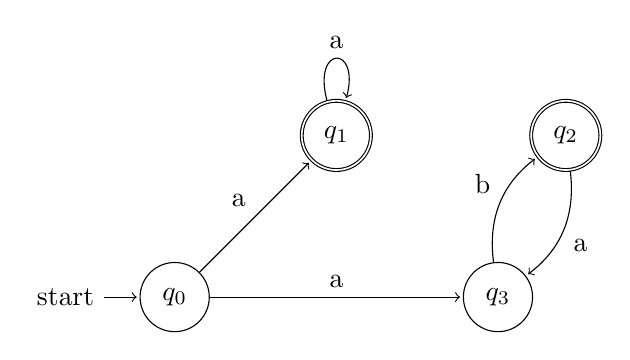
\begin{tikzpicture}[shorten >=1pt,node distance=2cm,auto] 
	\node[state,initial] (q_0)   {$q_0$}; 
	\node[state,accepting] (q_1) [above right=of q_0] {$q_1$}; 
	\node[state,accepting](q_2) [right=of q_1] {$q_2$};
	\node[state] (q_3) [below right=of q_1] {$q_3$}; 
	\path[->] 
	(q_0) edge  node {a} (q_1)
	edge node {a} (q_3)
	(q_1) edge [loop above] node {a} ()
	(q_2) edge [bend left]  node {a} (q_3)
	(q_3) edge [bend left]  node {b} (q_2);
	\end{tikzpicture}
	
	\question{2}{Finite-State Machines to Regex}
	
	\part{1} $ \varnothing^* $ (Rejecting any input)
	
	\part{2} $a^* + a^*b^+a^+b$ (Contains only $a$s or any pattern of $a$s to $b$s to $a$s to $b$s.)\\\\\\\\
	
	\question{3}{Binary Addition}
	
	$$A = \{w \in \Sigma^* \text{ $|$ } \text{ the bottom row of w is the sum of the top two rows } xy \in L_1 \}$$
	
	Prove that A is regular.
	
	{\em Proof}: 
	
	
	\question{4}{Division Operation?}
	
	$$\frac{L_1}{L_2} = \{x \text{ $|$ } \exists \in L_2 \text{ s.t. } xy \in L_1 \}$$
	Prove that if $L_1$ and $L_2$ are regular, then $\frac{L_1}{L_2}$ is also regular.
	
	{\em Proof}: 
	From a lemma, for every regular expression $R$, there is a DFA that recognizes the language $L(R)$.
	Suppose $L_1$ and $L_2$ are regular, then there exist DFA $M_1 =(Q,\Sigma,\delta,q_0,F_1)$ which accepts $L_1$ and DFA $M_2 =(Q,\Sigma,\delta,q_0,F_2)$ which accepts $L_2$. We want to show that $L_3 = \frac{L_1}{L_2}$ where $L_1, L_2, L_3 \in \mathbb{I}$.
	
	We have that $Q, \Sigma, \delta, \text{and } q_0$ in $M_1$ and $M_2$ can be shared, just that the accepting states are different. $L_3$ then can be recognized by some DFA $M_3 = (Q,\Sigma,\delta,q_0,F_3)$. We know that $\Sigma$ is a number digit alphabet (0-9). Then, each state is just an integer. So, $\forall x \in F_1, \exists y \in F_2, \text{and } \exists z \in F_3, zy = x$.
	
	From the observation, $L_1$, which is regular, contains accepting states that made of $zy$ from $F_2$ and $F_3$. Also, $L_2$, which is regular, recognized by $M_2$ and we can choose any number to be an accepting state in $F_2$ (As long as we accept at least a number). Since $F_3$ can be any state (number) also, there always exist $z$ that will satisfied $zy = x$. Thus, $M_3$ exists since we can design $F_3$.
	
	Therefore, if $L_1$ and $L_2$ are regular, then $\frac{L_1}{L_2}$ is also regular. $\square$
	
	\question{5}{Does It Accept Everything?}
	Let $M = (Q, \Sigma, \delta, q_0, F)$.
	
	\part{1} DFS could be a solution
	\\\\\\\\\\\\\\\\\\\\\\\\\\
	
	
	\question{6}{All The Same?}
	\part{1} 
	
	\part{2} 
	
	\part{3}
\end{document}